%%%%%%%%%%%%%%%%%%%%%%%%%%%%%%%%%%%%%%
% Main Preamble
%%%%%%%%%%%%%%%%%%%%%%%%%%%%%%%%%%%%%%
\documentclass[10pt]{article}
\usepackage{fullpage}
\usepackage{amsfonts}
\usepackage{amsmath}
\usepackage{amsthm}
\usepackage{graphicx}
\usepackage{color}
\usepackage{amssymb}
\usepackage{empheq}
\usepackage{mathrsfs}
\usepackage{enumerate}
\usepackage{tikz}
\usepackage{pgflibraryarrows}
\usepackage{pgflibrarysnakes}
\usepackage{upgreek}
\usepackage{tipa}
\usepackage{multicol}
\usepackage{verbatim}
\usepackage{floatrow}
\usepackage{gensymb}
\usepackage{caption}

\usepackage[T1]{fontenc}
\usepackage[font=small,labelfont=bf,tableposition=top]{caption}

\DeclareCaptionLabelFormat{andtable}{#1~#2  \&  \tablename~\thetable}

%%%%%%%%%%%%%%%%%%%%%%%%%%%%%%%%%%%%%%
% Header/footer
%%%%%%%%%%%%%%%%%%%%%%%%%%%%%%%%%%%%%%
\usepackage{fancyhdr}
\setlength{\headheight}{15.2pt}
\pagestyle{fancy}
\setlength\headsep{30pt}
\lhead{P2.WS1}
\rhead{Kutztown University -- MATH 210}
\fancyfoot{}

%%%%%%%%%%%%%%%%%%%%%%%%%%%%%%%%%%%%%%
% Document
%%%%%%%%%%%%%%%%%%%%%%%%%%%%%%%%%%%%%%
\begin{document}

\begin{center}
\Large{\textsc{Phase 2 (part 1): Solving Linear Systems of Equations}}\\
\end{center}

\begin{enumerate}[{$1.]$}]
\item Consider the following linear system:
\begin{align*}
	x - 2y  &= 1 \\ 
	x + 2y &= 5 \end{align*}

\begin{enumerate}[{$a.)$}]
\item Solve the linear system for $x$ and $y$ using elimination.  Then, graph each line below to confirm the solution is correct.

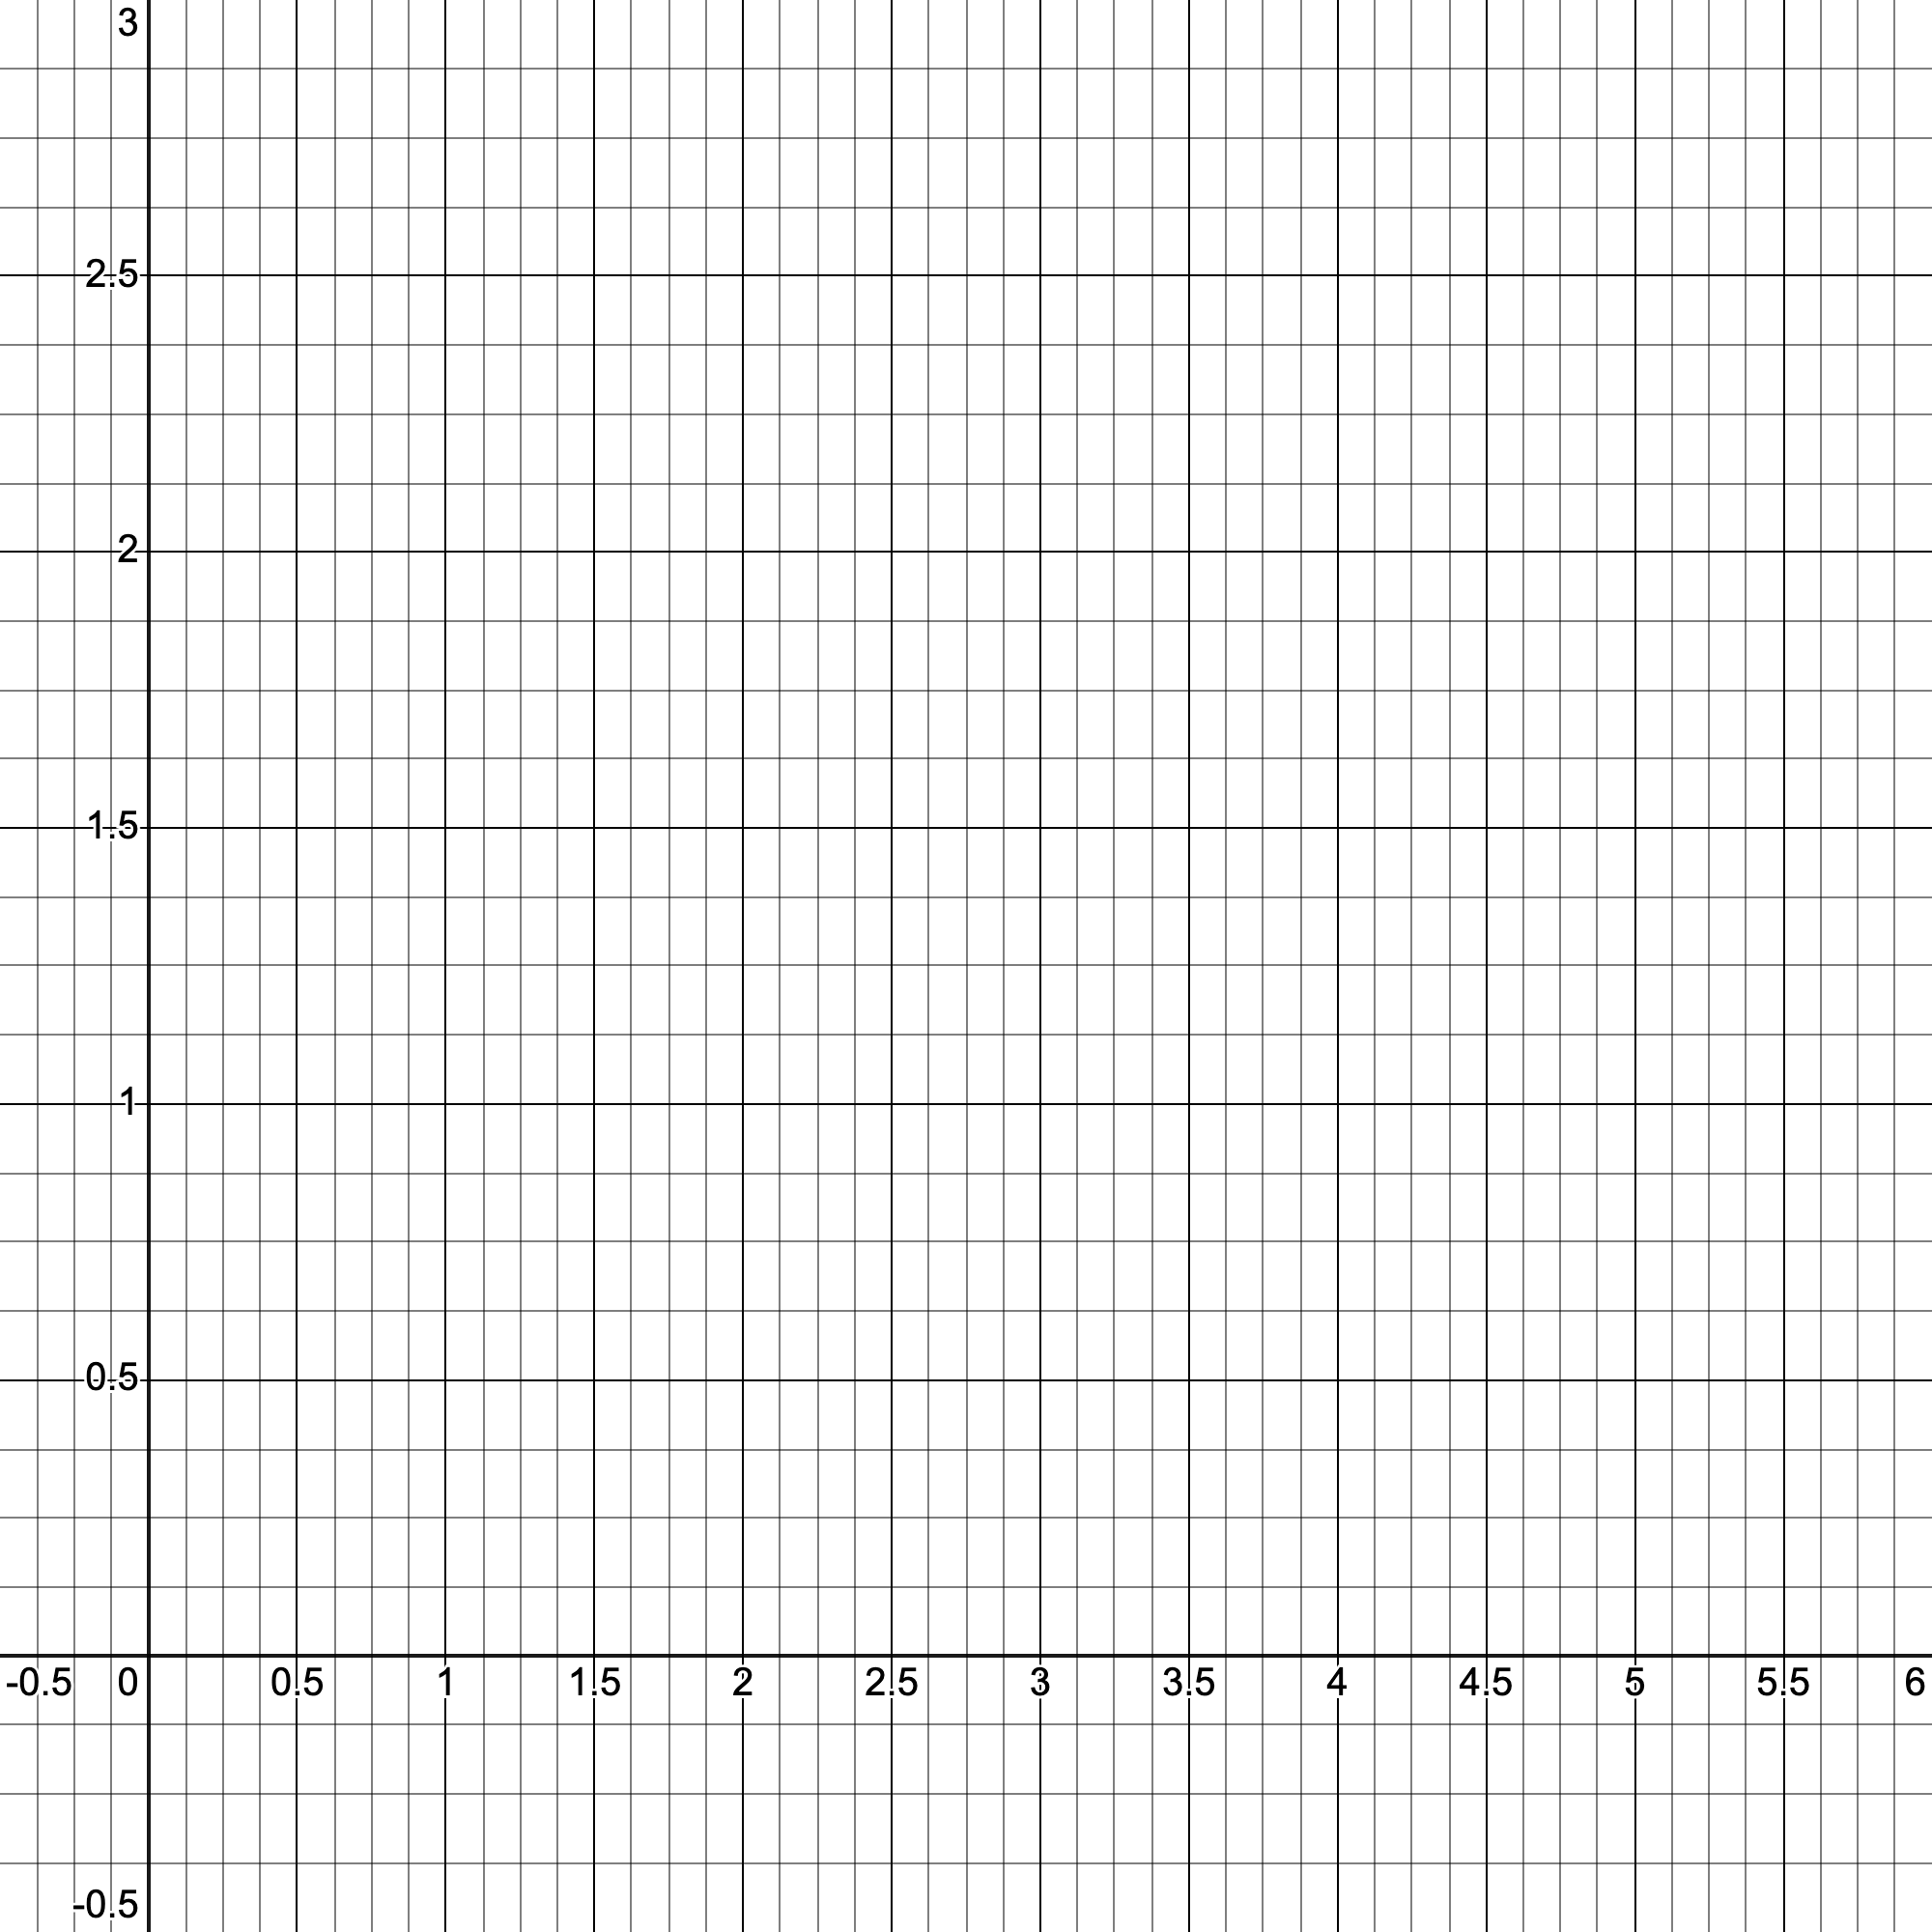
\includegraphics[width = .5\textwidth]{p2ws1_figure_1.png}

\item Write the system as a linear combination, and confirm that the solution above is correct. Sketch the original vectors below and linear combination of the vectors on the plane below: 

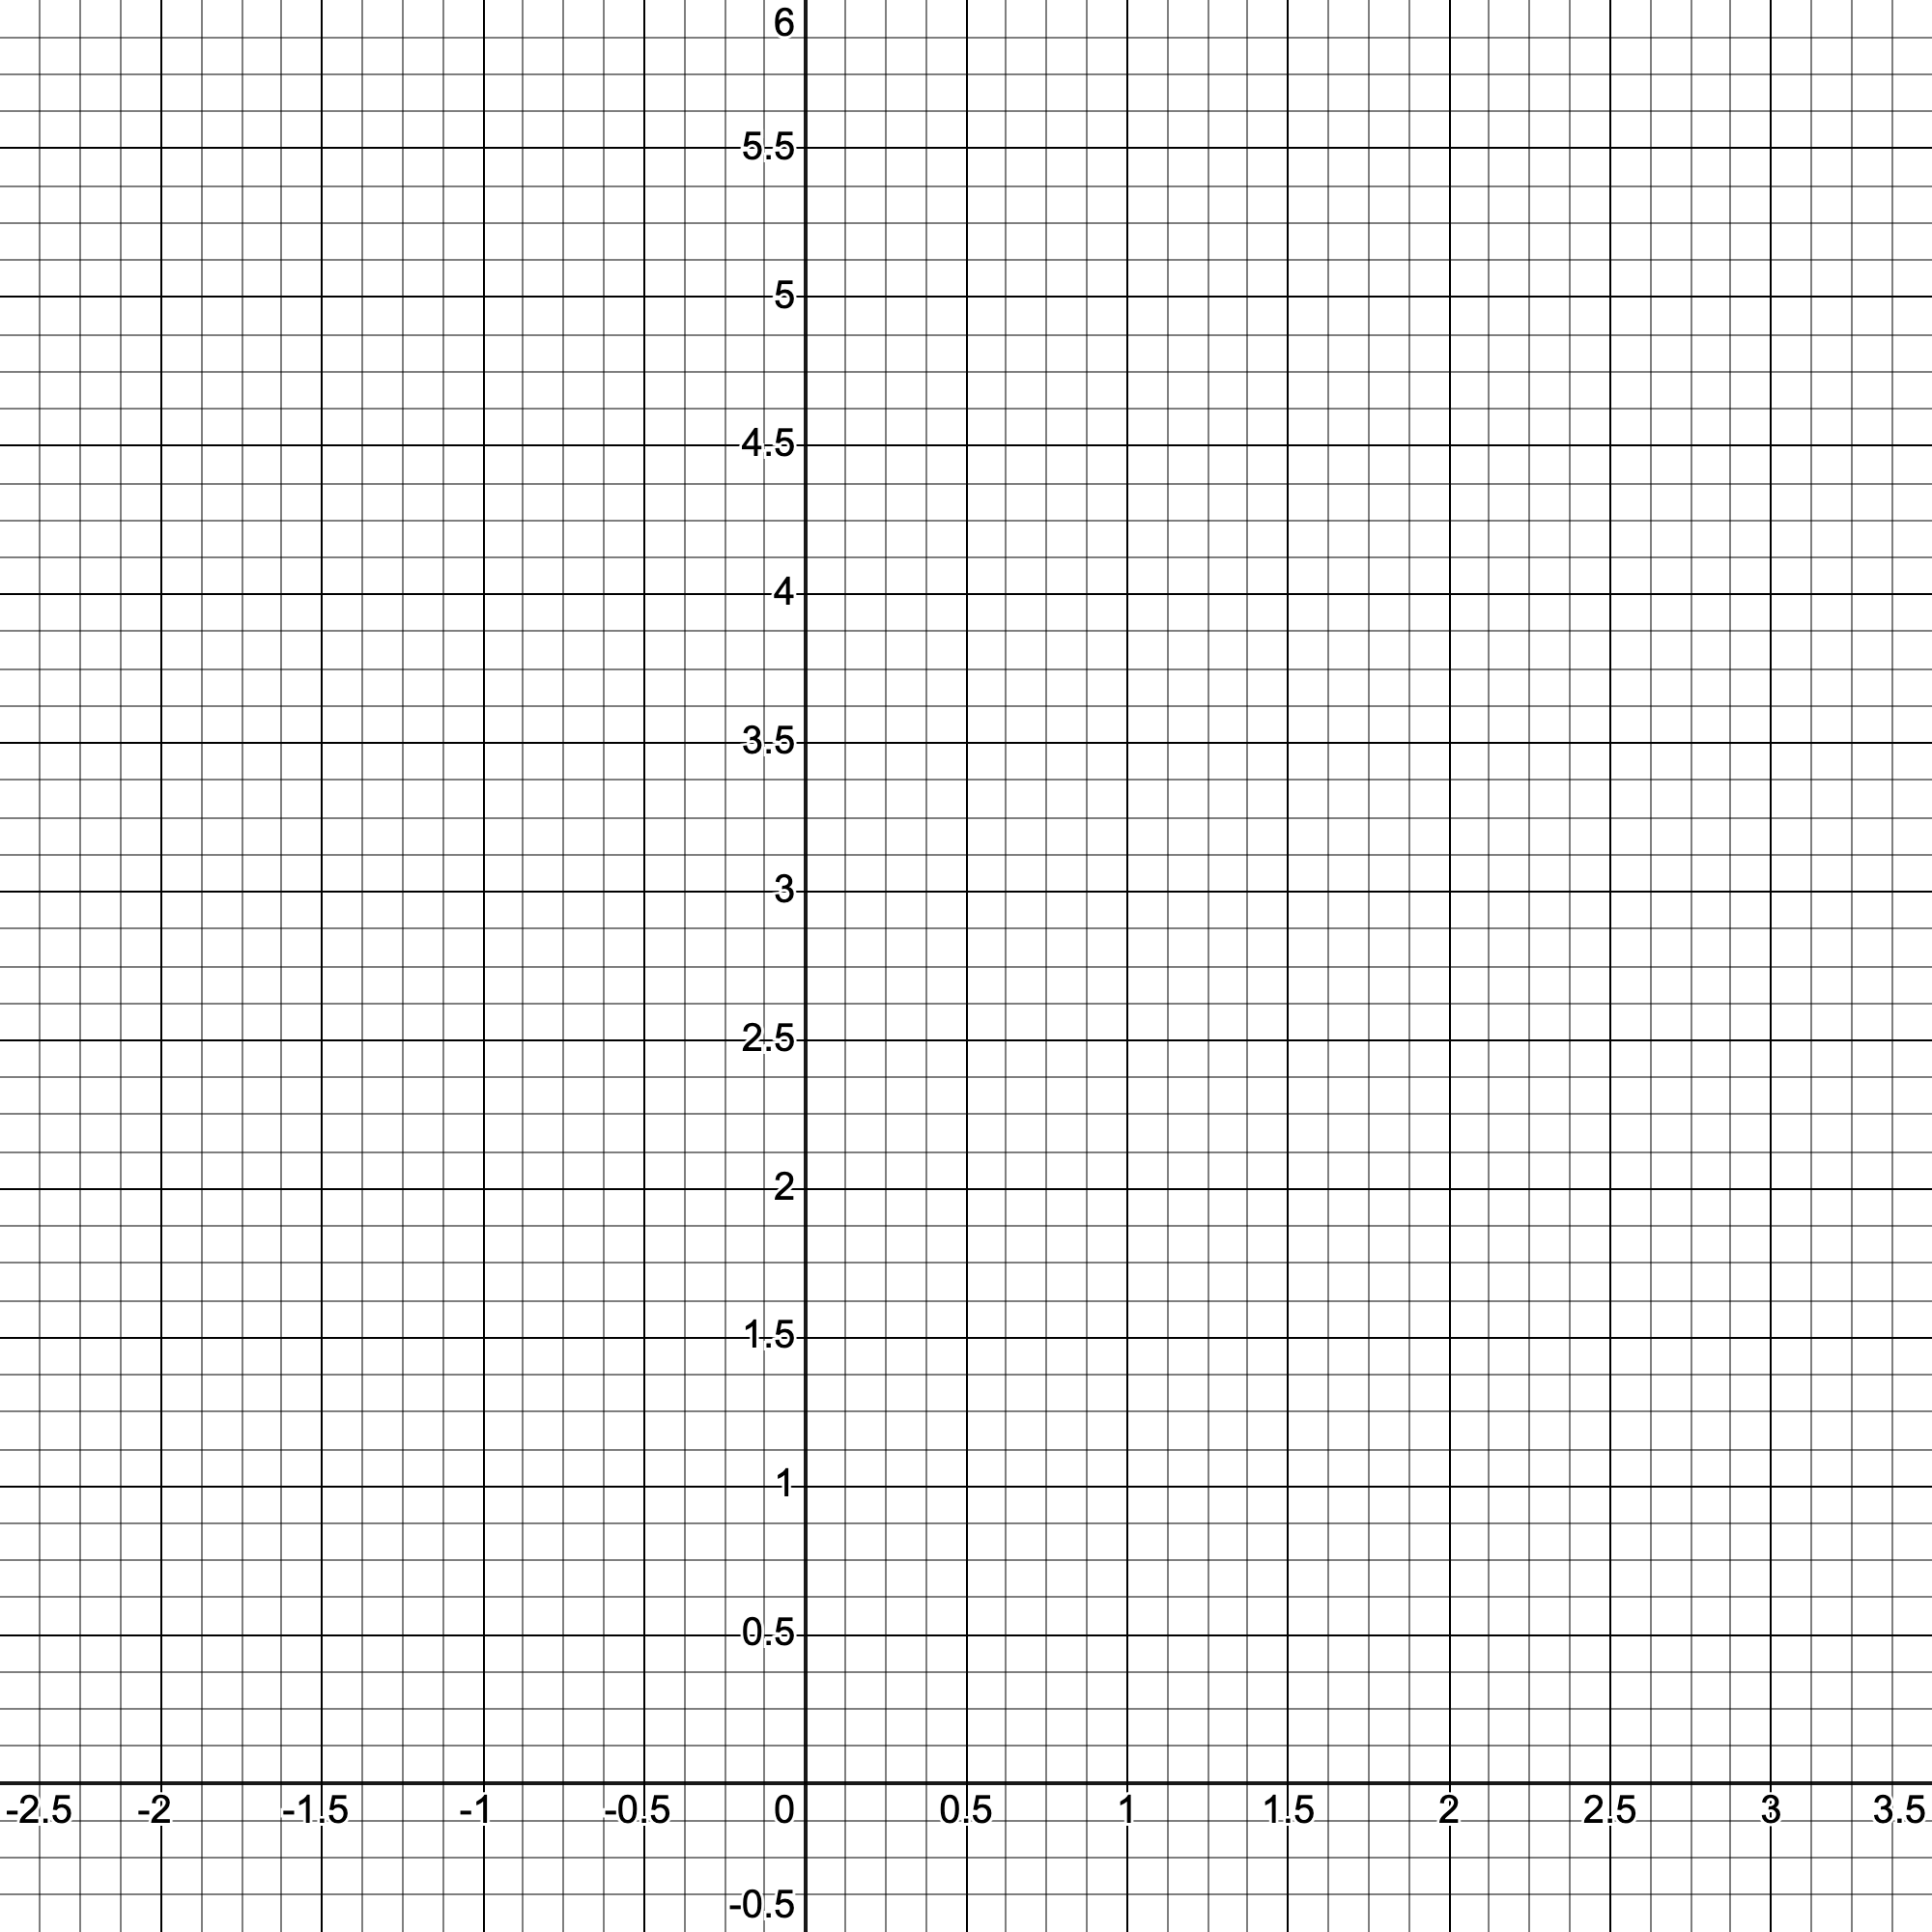
\includegraphics[width = .5\textwidth]{p2ws1_figure_2.png}

\end{enumerate}




\pagebreak


\item Suppose we want to find the equation of the line $y = mx + b$ that goes through the points $(1,-3)$ and $(-4,5)$.  Find the equation of the line by first formulating the problem as a $2 \times 2$ linear system of equations.  Then, solve it in Python and plot the solution along with the two points to show that the line goes through the points. \vfill

\item Suppose we want to find the equation of the plane $z = m_1x + m_2y + b$ that goes through the points $(1,-3,2)$ and $(-4,5,1)$, and $(0,3,1)$.  Find the equation of the plane by first formulating the problem as a $3 \times 3$ linear system of equations.  Then, solve it in Python and plot the solution along with the three points to show that the line goes through the points. \vfill\vfill



\end{enumerate}

\end{document}